\documentclass[border=6pt]{standalone}
\usepackage{mathptmx}
\usepackage{tikz}
\usetikzlibrary{positioning,arrows.meta}
\begin{document}
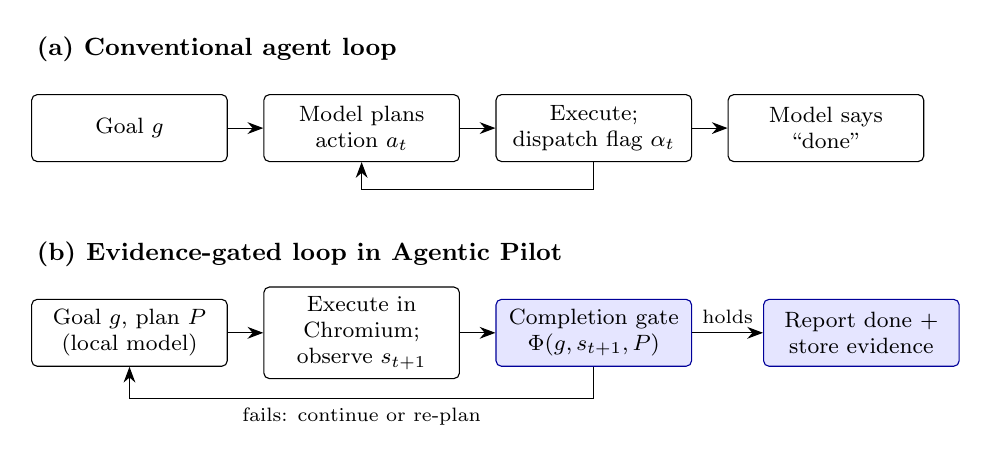
\begin{tikzpicture}[font=\footnotesize,
  box/.style={draw,rounded corners=2pt,minimum height=0.85cm,text width=2.25cm,align=center},
  gate/.style={box,fill=blue!10,draw=blue!60!black},
  arr/.style={-{Stealth[length=2mm]}}]
\node[font=\small\bfseries,anchor=west] at (-1.3,1.0) {(a) Conventional agent loop};
\node[box] (a1) at (0,0) {Goal $g$};
\node[box,right=0.45cm of a1] (a2) {Model plans action $a_t$};
\node[box,right=0.45cm of a2] (a3) {Execute; dispatch flag $\alpha_t$};
\node[box,right=0.45cm of a3] (a4) {Model says ``done''};
\draw[arr] (a1)--(a2); \draw[arr] (a2)--(a3); \draw[arr] (a3)--(a4);
\draw[arr] (a3.south) -- ++(0,-0.35) -| (a2.south);
\node[font=\small\bfseries,anchor=west] at (-1.3,-1.6) {(b) Evidence-gated loop in Agentic Pilot};
\node[box] (b1) at (0,-2.6) {Goal $g$, plan $P$ (local model)};
\node[box,right=0.45cm of b1] (b2) {Execute in Chromium; observe $s_{t+1}$};
\node[gate,right=0.45cm of b2] (b3) {Completion gate $\Phi(g,s_{t+1},P)$};
\node[gate,right=0.9cm of b3] (b4) {Report done + store evidence};
\draw[arr] (b1)--(b2); \draw[arr] (b2)--(b3); \draw[arr] (b3)--node[above,font=\scriptsize]{holds}(b4);
\draw[arr] (b3.south) -- ++(0,-0.4) -| node[pos=0.25,below,font=\scriptsize]{fails: continue or re-plan} (b1.south);
\end{tikzpicture}
\end{document}
